\section{Vendor Lock-In}

\subsection{Form \& Causes}
In general it is strong dependence on a particular vendor technology which makes difficult or expensive to switch to an other technology \cite{Definition}. This especially problem when using vendors technology which is not based on global or open standards \cite{c2comVendor}. Each vendor update or change make problems to continuously maintain system interoperability \cite{SurvivalGuide}.

One of causes of this anti-patter is selecting product basing on marketing or sales information instead of technology inspection. Selected product varies from published open system standards because there is no conformance process which leads need for deep in knowledge about the product. Also thigh coupling with vendor technology is always bad practice - avoiding of developing isolation layer \cite{SurvivalGuide}.

\subsection{Symptoms \& Consequences}

Depending upon vendor technology will drive application maintenance cycle. This can evolve to the problem when promised product features are delayed or never delivered because of vendor failures. In other hand missing product update will often end up on complete reintegration from the beginning \cite{SurvivalGuide}.
Attempts to change vendor technology is costly, difficult or impossible because of market monopoly.

\subsection{Example}

Typical example on software level are file formats. File formats that are not easily convertible to other formats will force they users to stick with one software that is able to use it \cite{Definition}. Real world example will be Microsoft Word, Outlook and Excel \cite{VendorWiki}.


\subsection[Solution]{Solution*}

\footnote{Due to lack of other source the whole chapter is based on \cite{SurvivalGuide}}
To avoid problems with changing vendor technology or to deal with vendor software updates problem and isolation layer should be provided. It should be used in cases when vendor technology is low level one or there is need to provided more convenient programming interface is necessary.

\begin{figure}[!h]
    \centering
    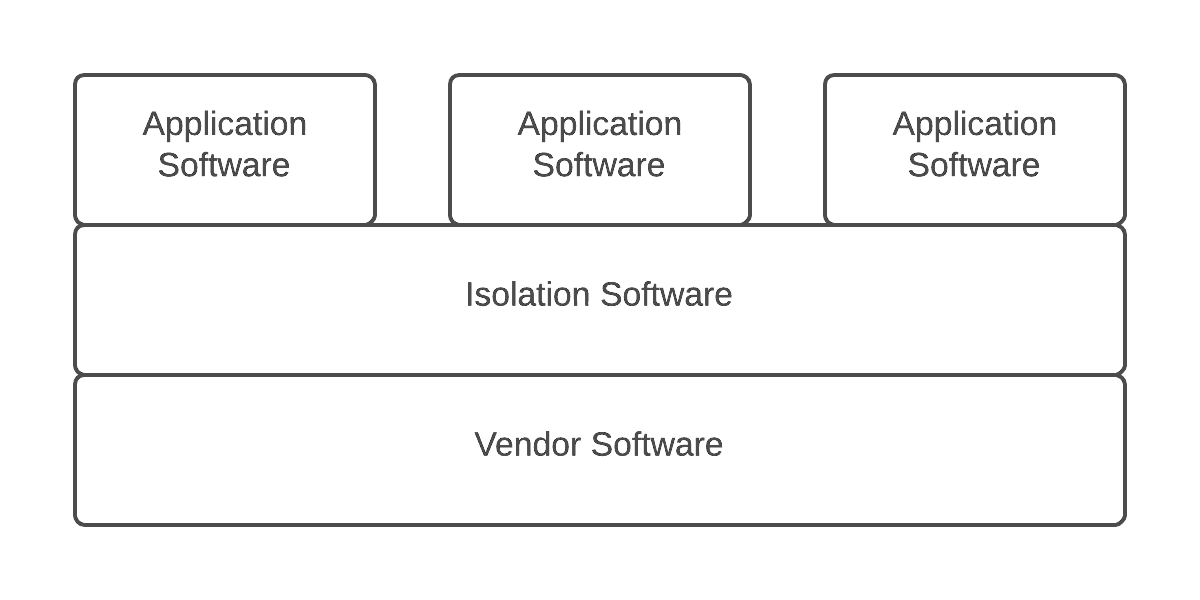
\includegraphics[scale=0.3]{Images/vendorsolution.png}
    \caption[Vendor Lock-In Isolation Layer]{Vendor Lock-In Isolation Layer \cite{SurvivalGuide}}
    \label{fig:vendorsolution}
\end{figure}

This layer can and should provided following functionalities:
\begin{itemize}
\item Handling default behaviors
\item Errors handling
\item Cross platform/system interface
\item Version inspection
\item Types and formats conversions
\end{itemize}
Benefits from this solution are such that migration of the system to an other vendor will not require changes in systems but only in isolation layer. This will lower costs and risks of such operation. There is also separation of infrastructure, low level knowledge from application knowledge which allows one team to maintain isolation layer and all others to develop applications without facing all problems connected with vendor product.

But isolation layer has to be maintained and coordinated. Requires additional development effort and can produce additional problems. While designing developers must be coordinated to avoid stovepipe enterprise anti-pattern.

\subsection{Exceptions}

This anit-pattern can be acceptable when a single vendor's code makes up the majority of code needed in an application \cite{SurvivalGuide}. Also when the whole enterprise is using the same (but not low level) technology provided by single strong company it will many not cause problems related to this vendor lock-in anti-pattern. 